\documentclass{sig-alternate}
\usepackage[latin1]{inputenc}
\usepackage{graphicx}        % standard LaTeX graphics tool
\usepackage{url} 
\usepackage{listings}
\usepackage{color}

\usepackage{color}
\usepackage{alltt}
\usepackage[T1]{fontenc}

% Style definition file generated by highlight 2.9, http://www.andre-simon.de/ 

% Highlighting theme definition: 

\newcommand{\hlstd}[1]{\textcolor[rgb]{0,0,0}{#1}}
\newcommand{\hlnum}[1]{\textcolor[rgb]{0.5,0,0.5}{\bf{#1}}}
\newcommand{\hlesc}[1]{\textcolor[rgb]{1,0,1}{\bf{#1}}}
\newcommand{\hlstr}[1]{\textcolor[rgb]{0.65,0.52,0}{#1}}
\newcommand{\hlpps}[1]{\textcolor[rgb]{0,0,1}{#1}}
\newcommand{\hlslc}[1]{\textcolor[rgb]{0.95,0.47,0}{#1}}
\newcommand{\hlcom}[1]{\textcolor[rgb]{1,0.5,0}{#1}}
\newcommand{\hlppc}[1]{\textcolor[rgb]{0,0.5,0.75}{\bf{#1}}}
\newcommand{\hlopt}[1]{\textcolor[rgb]{1,0,0.5}{\bf{#1}}}
\newcommand{\hlipl}[1]{\textcolor[rgb]{0.62,0.36,1}{#1}}
\newcommand{\hllin}[1]{\textcolor[rgb]{0.19,0.19,0.19}{#1}}
\newcommand{\hlkwa}[1]{\textcolor[rgb]{0.73,0.47,0.47}{\bf{#1}}}
\newcommand{\hlkwb}[1]{\textcolor[rgb]{0.5,0.5,0.75}{\bf{#1}}}
\newcommand{\hlkwc}[1]{\textcolor[rgb]{0,0.5,0.75}{#1}}
\newcommand{\hlkwd}[1]{\textcolor[rgb]{0,0.27,0.4}{#1}}
\definecolor{bgcolor}{rgb}{0.93,0.93,0.93}

%Comentario mielda para arreglar el git
\lstset{
basicstyle=\ttfamily \scriptsize,
language=java,
frame=single,
stringstyle=\ttfamily,
showstringspaces=false
}


\providecommand{\e}[1]{\ensuremath{\times 10^{#1}}}
\begin{document}
%
% --- Author Metadata here ---
\conferenceinfo{GECCO'13 Companion,} {July 6--10, 2013, Amsterdam, The Netherlands.} 
\CopyrightYear{2013} 
\crdata{978-1-4503-1964-5/13/07} 
\clubpenalty=10000 
\widowpenalty = 10000

\title{Developing Services in a Service Oriented Architecture for Evolutionary Algorithms}

%\subtitle{[Extended Abstract]
%\titlenote{A full version of this paper is available as
%\textit{Author's Guide to Preparing ACM SIG Proceedings Using
%\LaTeX$2_\epsilon$\ and BibTeX} at
%\texttt{www.acm.org/eaddress.htm}}}
%
% You need the command \numberofauthors to handle the 'placement
% and alignment' of the authors beneath the title.
%
% For aesthetic reasons, we recommend 'three authors at a time'
% i.e. three 'name/affiliation blocks' be placed beneath the title.
%
% NOTE: You are NOT restricted in how many 'rows' of
% "name/affiliations" may appear. We just ask that you restrict
% the number of 'columns' to three.
%
% Because of the available 'opening page real-estate'
% we ask you to refrain from putting more than six authors
% (two rows with three columns) beneath the article title.
% More than six makes the first-page appear very cluttered indeed.
%
% Use the \alignauthor commands to handle the names
% and affiliations for an 'aesthetic maximum' of six authors.
% Add names, affiliations, addresses for
% the seventh etc. author(s) as the argument for the
% \additionalauthors command.
% These 'additional authors' will be output/set for you
% without further effort on your part as the last section in
% the body of your article BEFORE References or any Appendices.


%\numberofauthors{1}
% \author{
% \alignauthor
% P. Garc{\'i}a-S{\'a}nchez, M. G. Arenas, P. A. Castillo, C. Fernandes, J. Gonz{\'a}lez, A.M. Mora and J.J. Merelo}\\
%        \affaddr{Department of Computer Architecture and Computer Technology and CITIC-UGR}\\
%        \affaddr{ETS. Inform{\'a}tica y Telecomunicaci{\'o}n}\\
%        \affaddr{University of Granada, Spain}\\
%        \email{pgarcia@atc.ugr.es}
% }
% }
 %\alignauthor
 %Anonymous\\
 %\affaddr{Lost island}\\
 %\affaddr{Unknown}\\
 %\affaddr{Pacific Ocean}\\
 %\email{lock@lost.com}
 

\numberofauthors{1}
 \author{
 \alignauthor
 Pablo Garc{\'i}a-S{\'a}nchez, Mar{\'i}a Isabel Garc{\'i}a Arenas, Antonio Miguel Mora, Pedro {\'A}ngel Castillo, Carlos Fernandes, Paloma de las Cuevas, Gustavo Romero, Jes{\'u}s Gonz{\'a}lez and Juan Juli{\'a}n Merelo\\
        \affaddr{University of Granada}\\
        \affaddr{Department of Computer Architecture and Computer Technology, ETSIIT and CITIC-UGR}\\
        \affaddr{18071 - Granada, Spain}\\
        \email{pgarcia@atc.ugr.es}
 }


%\numberofauthors{4} %  in this sample file, there are a *total*
% of EIGHT authors. SIX appear on the 'first-page' (for formatting
% reasons) and the remaining two appear in the \additionalauthors section.
%

%\author{
% You can go ahead and credit any number of authors here,
% e.g. one 'row of three' or two rows (consisting of one row of three
% and a second row of one, two or three).
%
% The command \alignauthor (no curly braces needed) should
% precede each author name, affiliation/snail-mail address and
% e-mail address. Additionally, tag each line of
% affiliation/address with \affaddr, and tag the
% e-mail address with \email.
%
% 1st. author
%\alignauthor
%Jack\\
%       \affaddr{Lost island}\\
%       \affaddr{unknow}\\
%       \affaddr{Pacific Ocean}\\
%       \email{jack_the_doctor@lost.com}
% 2nd. author
%\alignauthor
%Sawyer\\
%       \affaddr{Lost island}\\
%       \affaddr{unknow}\\
%       \affaddr{Pacific Ocean}\\
%       \email{sawyer_tom@lost.com}
% 3rd. author
%\alignauthor 
%Lock\\
%       \affaddr{Lost island}\\
%       \affaddr{unknow}\\
%       \affaddr{Pacific Ocean}\\
%       \email{lock@lost.com}
% 4rd. author
%\alignauthor 
%Hurley\\
%       \affaddr{Lost island}\\
%       \affaddr{unknow}\\
%       \affaddr{Pacific Ocean}\\
%       \email{hugo@lost.com}
%}

%\and  % use '\and' if you need 'another row' of author names
% 4th. author
%\alignauthor Lawrence P. Leipuner\\
%       \affaddr{Brookhaven Laboratories}\\
%       \affaddr{Brookhaven National Lab}\\
%       \affaddr{P.O. Box 5000}\\
%       \email{lleipuner@researchlabs.org}
% 5th. author
%\alignauthor Sean Fogarty\\
%       \affaddr{NASA Ames Research Center}\\
%       \affaddr{Moffett Field}\\
%       \affaddr{California 94035}\\
%       \email{fogartys@amesres.org}
% 6th. author
%\alignauthor Charles Palmer\\
%       \affaddr{Palmer Research Laboratories}\\
%       \affaddr{8600 Datapoint Drive}\\
%       \affaddr{San Antonio, Texas 78229}\\
%       \email{cpalmer@prl.com}
%}
% There's nothing stopping you putting the seventh, eighth, etc.
% author on the opening page (as the 'third row') but we ask,
% for aesthetic reasons that you place these 'additional authors'
% in the \additional authors block, viz.
%\additionalauthors{Additional authors: John Smith (The Th{\o}rv{\"a}ld Group,
%email: {\texttt{jsmith@affiliation.org}}) and Julius P.~Kumquat
%(The Kumquat Consortium, email: {\texttt{jpkumquat@consortium.net}}).}
%\date{30 July 1999}
% Just remember to make sure that the TOTAL number of authors
% is the number that will appear on the first page PLUS the
% number that will appear in the \additionalauthors section.

\maketitle

\begin{abstract}
This paper shows the design and implementation of services for Evolutionary Computation following the Service Oriented Architecture paradigm. This paradigm allows independence over language and distribution mechanism. This development is challenging because some technological and design issues, such as abstract design or unordered execution. To solve them, OSGiLiath, an implementation of an abstract Service Oriented Architecture for Evolutionary Algorithms, is used to develop new interoperable services taking into account these restrictions.  
\end{abstract}

% A category with the (minimum) three required fields
%\category{H.4}{Information Systems Applications}{Miscellaneous}
%A category including the fourth, optional field follows...
\category{D.2.11}{Software Engineering}{Software Architectures}[Data abstraction]
\category{D.2.12}{Software Engineering}{Interoperability}[Distributed objects]
\category{I.2.8}{Artificial Intelligence}{Problem Solving, Control Methods, and Search}[Heuristic methods]

%sures, performance measures
\terms{Algorithms}


\keywords{Service oriented architecture, evolutionary algorithms, genetic algorithms, distributed algorithms, OSGi}


%
%%%%%%%%%%%%%%%%%%%%%%%%%%%%%%%   INTRODUCTION   %%%%%%%%%%%%%%%%%%%%%%%%%%%%%%%
%
\section{Introduction}
\label{sec:intro}
%

%%CAMBIAR ESTO
Service Oriented Architecture (SOA) \cite{PAPAZOGLOU} is becoming an important trend in software development. This paradigm allows the organization and distribution using the {\em service} concept. A service is an interaction depicted in Figure \ref{SOADIAGRAM}. The service provider publishes {\em service descriptions} (or interfaces) in the {\em service registry}, so the {\em service requesters} can discover services and bind to the {\em service providers} to use it.

SOA allows independence in language and distribution mechanisms, aiming to easy extension and integration, but it has the following restrictions:

\begin{itemize}
\item Services must be input/output functions.
\item The services must not have state (i.e. not global variables).
\item The order of execution of the services is not defined.
\item Services must be designed as abstract as possible.
\end{itemize}

Distributed computing offers the possibility of taking advantage of parallel processing,
 in order to obtain a higher 
computing power \cite{OPENSCIENCEGRID}.
 SOA is also applied in this area, using platforms based on Web Services \cite{PAPAZOGLOU}, and new standards for this paradigm have emerged, like OSGi (Open Services Gateway Initiative) \cite{OSGI}.


OSGi allows build quality software systems considering a high level of modularity. Besides the benefits that classic
modularization paradigms can offer (like object-oriented modelling),
and the improvements in test, reusability, availability and
maintainability, it is necessary to explore other modelling techniques, such as the
plug-in based development and the SOA design. This kind of development
simplifies aspects such as the complexity, personalization, configuration,
development and cost of the software development. In the optimization
heuristics software area, the benefits that using this kind of
development can offer are carried out in the development of algorithms,
experimental evaluation, and combination of different optimization
paradigms \cite{PLUGINS}.  





\begin{figure}[ht] 
\begin{center} 
 % \epsfig{file=soaDiagram.eps,width=7.5cm} 
\includegraphics[scale=1]{images/soaDiagram.eps}
\end{center} 
\caption{Service interaction schema. The service provider publish a service description that is used by the requestor to find and use services.} 
\label{SOADIAGRAM} 
\end{figure} 







In our previous work \cite{OSGILIATH} we presented an abstract Service Oriented Architecture for Evolutionary Algorithms (SOA-EA), with guidelines and steps to migrate from traditional development in Evolutionary Algorithms (EAs) to SOA. It also presented a specific implementation, called OSGiLiath ({\em OSGi Laboratory for Implementation and Testing of Heuristics}): an environment for the development of distributed algorithms extensible via plug-ins architecture and based in a wide-accepted software specification (OSGi). In this work, a full service development is presented, taking into account the specific technology used, instead an abstract design, as in our previous work.

%Therefore, the objective of the proposed environment in this paper is to facilitate the
%development of distributed computing applications by using the OSGi standard,
%taking advantage
%of the plug-in software development and SOA that can compete with existing
%distributed applications in easy of use, compatibility and development.
The rest of the work is structured as follows: after the state of
the art, we present design principles to create services for Evolutionary Computation (Section \ref{sec:design}). Then, the OSGi implementation technology is explained in Section \ref{sec:technology}, used to build our framework (described in Section \ref{sec:osgiliath}). Then, the steps to create services with this framework are explained (Section \ref{sec:development}). Finally, conclusions and suggestions for future work are presented (Section \ref{sec:conclusions}).


%%%%%%%%%%%%%%%%%%%%%%%%%%%%%%  SOA  %%%%%%%%%%%%%%%%%%%%%%%%%%%%%%
%
\section{State of the art}
\label{sec:soa}
%
Even as SOA is used extensively in software development, it is not widely accepted in the EA community. Most of the frameworks have the lack of low generality, because they
are focused in a specific field, like EasyLocal++ \cite{EASYLOCAL} (focused in Local Search) or
SIGMA \cite{SIGMA} (in the field of optimization-based decision support systems). Another common issue is that they are just libraries
 or Perl modules \cite{PERL}, they have no GUIs, or they are complicated to
install and require many programming skills. Another problem could be
the lack of comfort, for example, C++ has a more complicate sintaxis
than other languages. There also exist frameworks that use metaheuristics to apply in specific fields, like the KEEL framework \cite{KEEL}, that let the creation of heuristics to apply in data-mining problems.

Among this great number of software tools we want to focus in the most widely accepted distributed algorithms frameworks. ECJ \cite{ECJ}, Evolutionary Computation in Java, is a set of Java classes that can be extended and includes several communication modules. MALLBA \cite{MALLBA} is based in software skelletons with a common and public interface. Every skeleton implements a resolution technique for optimization in the fields of exact, heuristic or hybrid optimization. It provides LAN and WAN capacity distribution with MPI . However, this both frameworks are not based in the plug-in development, so they can not take advantage of features like the life-cycle management, versioning, or dynamic service binding, as OSGi proposes.

Another important platform is DREAM \cite{DREAM}, which is an open source framework for Evolutionary Algorithms based on Java that
defines an island model and uses the Gossip protocol and TCP/IP sockets for
communication. It can be deployed in P2P platforms and it is divided
in five layers. Every layer provides an user interface and different
interaction and abstraction level, but adding new functionalities is not so easy, due to the the fact that system must be stopped before adding new modules and the implementation of interfaces must be defined in the source code, so a new compilation is needed (as in ECJ). OSGi lets the addition of new functionalities only compiling the new features, not the existing ones. 

The MALLBA authors are now working in the jMetal Framework \cite{JMETAL}, that is a newer Java-based framework, but it has not yet distributed capabilities and it is focused in multi-objective optimization.

ParadiseEO \cite{PARADISEO} allows the design of Evolutionary Algorithms and Local Search with hybridization, providing a variety of operators and evaluation functions. It also implement the most common parallel and distributed models, and it is based in standard libraries like MPI, PVM and Pthreads. However, it has the same problems that the previous frameworks, not lifecycle management or service oriented programming. GAlib \cite{GALIB} is very similar and share the same characteristics and problems.

In the field of the plug-in based frameworks, HeuristicLab \cite{HEURISTICLAB} is the most outstanding example. It also allows the distributed programming using Web Services and a centralized database, instead using their own plug-in design for this distributed communication.

METCO framework \cite{METCO} also have the same problems, it does not use a standard plug-in system or SOA, but let the implementation of existing interfaces, and lets the user configure its existing functionalities.

Finally, the only service oriented optimization framework is GridUFO \cite{GRIDUFO}, but it only allows the modification of the objective function and the addition of whole algorithms, without combining existing services.

Previous frameworks are designed to be extensible and re-usable, but without taking into account the restrictions of SOA to achieve even more independence and development improvements.

\section{Designing Services for a Service Oriented Architecture for Evolutionary Algorithms}
\label{sec:design}

In \cite{OSGILIATH} we demonstrated that it is possible to create a service oriented architecture for EAs using a specific SOA technology. This architecture used the features that SOA offers. To do this, loose coupling services for EAs were designed (SOA-EA), and they were implemented using a SOA technology and compared with other frameworks. These services can be combined in several ways to obtain different algorithms (for example, from a canonical GA, a NSGA-II can been created just adding new services). Also several techniques were presented to combine existing services in a flexible way.



\subsection{Design principles}

%Services must match the technological requirements given in previous sub-section. However, other design restrictions must be taken into account, 

One of the main restrictions in SOA, appart from focusing in develop abstract services, is the stateless nature of services. Therefore, in SOA the services design must follow several guidelines.

First, as services are unaware of others, there must not be global variables in any part of the code. Services are listening, and waiting to be executed. For example, a fitness service with a counter that is increased each time is called (to stop the algorithm if a limit is reached, for example). If several (and different) algorithms are working in parallel, and calling this function at the same time the counter would not distinguish between algorithms, giving erroneous results. However, a service that maintains some kind of state is allowed, for example, a statistic service that read events from all the algorithms being executed at the same time, but this should be managed to avoid errors.

Also, a service must not be distinguishable from local or remote running in other node in the network. Every stage in the algorithm should be treated as service to be executed in local or in remote, even the {\em Population} or the {\em Parameters}. Mechanisms to ensure the correct data-sharing should be provided. Also, many implementations of the same service could exist at the same time (different implementations of {\em Crossover}, for example) and it should be correctly managed and used.

Moreover, a service is always a request-response function. For example, the fitness calculation must not be a method of the {\em Individual} implementation, but a function that receives a list of individuals and returns a list of the calculated fitness of that individuals. This allow things such as remote fitness calculation and distributed load balancing, impossible to perform if the fitness is a method of the {\em Individual} class.



Thinking as abstract as possible requires separate concepts such the order of recombination, and the crossover itself. Usually, after parent selection, individuals are crossed in order. However, if we need a different mechanism for mating (for example, using more than two parents, or parent selected several times) a duplication of effort is needed. That is the reason we should sepparate the concept {\em recombine} from {\em crossover}. 

Finally, we must not make assumptions about services previously executed or being executed next. For example, services such {\em Recombinator} or {\em Mutator} should return the individuals with their fitness already calculated. Usually this step is performed in the last stage of the generation, but if we require the individuals for other tasks: for example, a Local Search or a statistics collector to guide the algorithm.

\subsection{Other technological restrictions}

In \cite{OSGILIATH} we also presented the advantages of using SOA in Evolutionary Algorithms area: firstly, SOA fits with the genericity advantages in the development of software for EAs \cite{GENERICITY05} and adds new features, like language independence and  distribution mechanisms. It also allows the addition and removal of services in execution time without altering the general execution of the algorithm (that is, it is not mandatory to stop it or to add extra code to support new operators). This issue increases the interoperability between different software elements. Moreover, this allows easy code distribution: SOA does not require the use of a concrete implementation or library.

In this work, a new process development, explaining the specific technology used is presented. The services developed must match with the next technological restrictions:
\begin{itemize}
\item These services can dynamically bound to cha\-nge the needed EA aspects. 
\item The source code of  the basic EA services must not been re-written or re-compiled to achieve this task. 
\item New services can be added in execution time. 
\item No specific source code for a distribution must added, neither the existing source code of the services should be modified for this purpose (that is, changing distribution libraries must not add extra code in exisitng services).
\end{itemize}


\section{Implementation technology}
\label{sec:technology}
This section dives into some technical features of the OSGi platform, to guide the reader to understand the OSGiLiath framework in a deeper way, and to evaluate the advantages of using this features in the development of distributed algorithms to match with the previous restrictions.

The used technology, OSGi, was proposed by a consortium of more than
eighty companies in order to develop an infrastructure for the
deployment of service in heterogeneous network of devices, mainly
oriented to domotics \cite{GATEWAY}. Nowadays it defines a
specification for a Service Oriented Architecture for virtual
machines (VMs). It provides very desiderable features, like
packet abstraction, life-cycle management, packaging or versioning,
allowing significant reduction of the building, support and deployment
complexity of the applications. 

OSGi technology allows dynamic discovery of new components, to increase the collaboration and to minimize and manage the coupling
among modules. Moreover, the
OSGi Alliance has developed several standard component interfaces for
common usage patterns, like HTTP servers, configuration, logs, security,
management or XML management among others, whose implementations can
be obtained by third-parties. Nowadays there are some challenges 
in the OSGi development \cite{OSGICHALLENGES}, but they only affect the creation of very complex applications.

This advantages are not so
                               costly, as can be thought: the OSGi
                                framework can be implemented in a
                                {\em jar} file\footnote{A jar file is
                                a file that groups the compiled Java
                                files.} of 300KB. Also, and different
                                of the normal usage of Java, each
                                class pre-charges only the other
                                classes to use, not all. Also is
                                non-intrusive: the code to be
                                executed in OSGi can be executed
                                without it. Finally, from its
                                specification in 1998 has been widely
                                used as base in big projects: the
                                Eclipse IDE (Integrated Development
                                Environment) is built over OSGi, and
                                also big application servers
                               (Glassfish or IBM Websphere) or
                               residential gateways
                               \cite{GATEWAY}, among other
                               examples. 

\subsection{OSGi Architecture}
To understand how OSGi \cite{OSGI} works and which capabilities could offer to the OSGiLiath users it is necessary to understand how OSGi is built. OSGi has a layered model that is depicted in Figure \ref{fig:osgi-original}. The terms present in this Figure are:

\begin{itemize}
\item Bundles: Bundles are the OSGi components made by developers. Is a normal {\em jar} file including Java classes and interfaces with different MANIFEST.MF and extra files (such as the Service Descriptions).
\item Services: This layer connects bundles in a dynamic way by offering a publish-find-bind model.
\item Life-Cycle: The API to install, start, stop, update, and uninstall bundles.
\item Modules: This layer defines how a bundle can import and export code (using the MANIFEST.MF file).
\item Security: Security aspects are handled in this layer.
\item Execution Environment: Defines what methods and classes are available in a specific platform. For example, mobile devices have less Java classes due to performance constraints.
\end{itemize}



\begin{figure}[t] 
\begin{center} 
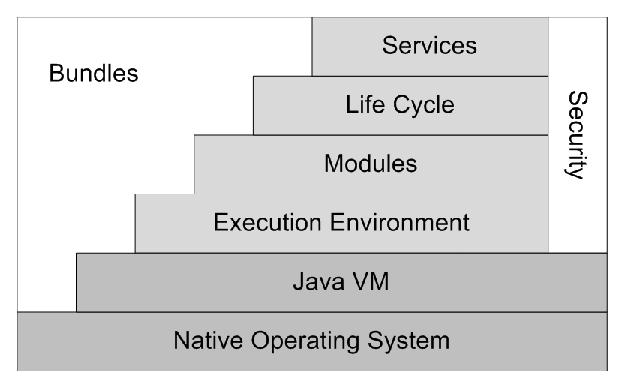
\includegraphics[scale=0.8]{images/osgi-oficial.eps} 
\end{center} 
\caption{OSGi layered architecture. Every layer is built from the one just below.} 
\label{fig:osgi-original} 
\end{figure}



\subsection{OSGi configuration files}
Regarding to explained OSGi layers how to use all OSGi capabilities is shown next. 

OSGi implements a dynamic component model, unlike normal Java
environments. Applications or components (also called
\emph{bundles}) can be remotely installed, started, stopped, updated
or uninstalled on the fly; moreover, the classes and
packaging management is specified in detail. The OSGi framework provides
APIs for the management of services that are exposed or used by the
bundles.

Java programmers are familiar with the {\em jar} concept. The first difference among a {\em bundle} and a {\em jar} is that the second has a MANIFEST.MF file adapted to be used in OSGi. This file indicates which clases imports or exports the {\em bundle}. An example can be seen in Figure \ref{fig:manifest}. This file shows the name of the bundle and its version (this is useful to select specific services), and the execution environment (that is, the Java Virtual Machine required). Also, this file specifies the XML files of the declarative services (in section {\em Service-Component}). However, this {\em bundle} can be used as a normal {\em jar} outside OSGi.

\begin{figure}[t]
\noindent
\ttfamily
\hlstd{}{\bf Manifest-Version:} 1.0\\
\hlstd{}{\bf Bundle-ManifestVersion:} 2\\
\hlstd{}{\bf Bundle-Name:} VRP\\
\hlstd{}{\bf Bundle-SymbolicName:} VRP\\
\hlstd{}{\bf Bundle-Version:} 1.0.0\\
\hlstd{}{\bf Bundle-RequiredExecutionEnvironment:} JAVA-1.6\\
\hlstd{}{\bf Import-Package:}  es.ugr.osgiliath,\\
 \hlstd{}  es.ugr.osgiliath.algorithms,\\
\hlstd{} es.ugr.osgiliath.events,\\
 \hlstd{}es.ugr.osgiliath.evolutionary,\\
 \hlstd{}es.ugr.osgiliath.evolutionary.basiccomponents.genomes,\\
 \hlstd{}es.ugr.osgiliath.evolutionary.basiccomponents.individuals,\\
 \hlstd{}es.ugr.osgiliath.evolutionary.elements,\\
 \hlstd{}es.ugr.osgiliath.evolutionary.individual,\\
 \hlstd{}es.ugr.osgiliath.evolutionary.migrator,\\
 \hlstd{}es.ugr.osgiliath.geneticalgorithm.distributed,\\
 \hlstd{}es.ugr.osgiliath.problem\\
\hlstd{}{\bf Export-Package:} es.ugr.osgiliath.vrp,\\
 \hlstd{}es.ugr.osgiliath.vrp.individual\\
\hlstd{}\hlkwa{Service-Component:} OSGI-INF/vrpinitializer.xml,\\
OSGI-INF/vrpfitnesscalculator.xml,\\
 OSGI-INF/vrpcrossover.xml,\\
 OSGI-INF/vrpmutation.xml\\
\mbox{}
 
\normalfont
\caption{Example of MANIFEST.MF. This example defines which packages are necessary to activate the bundle and which packages are exported.}
\label{fig:manifest}
\end {figure}





In normal environments, to create a specific implementation of an interface (i.e. {\em FitnessCalculator}) is as follows:

\begin{lstlisting}
class EvolutionaryAlgorithm implements Algorithm{
 FitnessCalculator fc;
 //A new instance is bound to a reference
 fc = new ExampleFunction();
}
\end{lstlisting}
 
With Declarative Services, the {\em new ExampleFunction()} part is not used, so if a new implementation is desired no code recompilation is necessary.  Figure \ref{fig:ds} shows a declarative service description file, which establish in execution time which implementation is bound to the interfaces. This example indicates that the implementation of service {\em FitnessCalculator} is {\em VRPFitnessCalculator}, but this service is not activated until all their references (other services, like {\em TransportData}) are also activated. The tag {\em cardinality} means that at least one service of that kind must exist (the first {\em 1} represents optionality) and  the second part (the other {\em 1} indicates the number of different implementations that can be managed: one ({\em 1}) or many ({\em *}).  We need to create XML files for the rest of services to expose (i.e. {\em TransportData}). The file where these capabilities are defined is declared in section {\em Service-Component} of MANIFEST.MF file, as can be seen in Figure \ref{fig:manifest}.
\begin{figure*}[t]
\noindent
\ttfamily
\hlstd{}\hlopt{$<$}\hlstd{?xml\ version}\hlopt{=}\hlstd{"}\hlnum{1.0}\hlstd{"\ encoding}\hlopt{=}\hlstd{"UTF{-}8"?}\hlopt{$>$}\hspace*{\fill}\\
\hlstd{}\hlopt{$<$}\hlstd{scr}\hlopt{:}\hlstd{component\ xmlns}\hlopt{:}\hlstd{scr}\hlopt{=}\hlstd{"http}\hlopt{://}\hlstd{www}\hlopt{.}\hlstd{osgi}\hlopt{.}\hlstd{org}\hlopt{/}\hlstd{xmlns}\hlopt{/}\hlstd{scr}\hlopt{/}\hlstd{v1}\hlopt{.}\hlstd{1}\hlnum{.0}\hlstd{"\ name}\hlopt{=}\hlstd{"VRPFitnessCalculator"}\hlopt{$>$}\hspace*{\fill}\\
\hlstd{}\hlstd{\ \ \ }\hlstd{}\hlopt{$<$}\hlstd{implementation\ class}\hlopt{=}\hlstd{"es}\hlopt{.}\hlstd{ugr}\hlopt{.}\hlstd{osgiliath}\hlopt{.}\hlstd{vrp}\hlopt{.}\hlstd{VRPFitnessCalculator"}\hlopt{/$>$}\hspace*{\fill}\\
\hlstd{}\hlstd{\ \ \ }\hlstd{}\hlopt{$<$}\hlstd{service}\hlopt{$>$}\hspace*{\fill}\\
\hlstd{}\hlstd{\ \ \ \ \ \ }\hlstd{}\hlopt{$<$}\hlstd{}\hlkwa{provide\ }\hlstd{interface}\hlopt{=}\hlstd{"es}\hlopt{.}\hlstd{ugr}\hlopt{.}\hlstd{osgiliath}\hlopt{.}\hlstd{evolutionary}\hlopt{.}\hlstd{elements}\hlopt{.}\hlstd{FitnessCalculator"}\hlopt{/$>$}\hspace*{\fill}\\
\hlstd{}\hlstd{\ \ \ }\hlstd{}\hlopt{$<$/}\hlstd{service}\hlopt{$>$}\hspace*{\fill}\\
\hlstd{}\hlstd{\ \ \ }\hlstd{}\hlopt{$<$}\hlstd{reference\ bind}\hlopt{=}\hlstd{"setTransportData"\ \hspace*{\fill}\\
}\hlstd{\ \ \ \ }\hlstd{unbind}\hlopt{=}\hlstd{"unsetTransportData"\hspace*{\fill}\\
}\hlstd{\ \ \ \ }\hlstd{cardinality}\hlopt{=}\hlstd{"}\hlnum{1}\hlstd{}\hlopt{.}\hlstd{}\hlnum{.1}\hlstd{"\ \hspace*{\fill}\\
}\hlstd{\ \ \ \ }\hlstd{interface}\hlopt{=}\hlstd{"es}\hlopt{.}\hlstd{ugr}\hlopt{.}\hlstd{osgiliath}\hlopt{.}\hlstd{vrp}\hlopt{.}\hlstd{TransportData"\ \hspace*{\fill}\\
}\hlstd{\ \ \ \ }\hlstd{name}\hlopt{=}\hlstd{"TransportData"\ \hspace*{\fill}\\
}\hlstd{\ \ \ \ }\hlstd{policy}\hlopt{=}\hlstd{"static"\hspace*{\fill}\\
}\hlstd{\ \ \ }\hlstd{}\hlopt{/$>$}\hspace*{\fill}\\
\hlstd{}\hlstd{\ \ \ }\hlstd{}\hlopt{$<$}\hlstd{property\ name}\hlopt{=}\hlstd{"name"\ }\hlkwa{type}\hlstd{}\hlopt{=}\hlstd{"String"\ }\hlkwa{value}\hlstd{}\hlopt{=}\hlstd{"vrpfitnesscalculator"}\hlopt{/$>$}\hspace*{\fill}\\
\hlstd{}\hlopt{$<$/}\hlstd{scr}\hlopt{:}\hlstd{component}\hlopt{$>$}\hlstd{}\hspace*{\fill}\\
\mbox{}
\normalfont
\caption{Service Description. This documents indicates that the implementation of the service {\em FitnessCalculator} is {\em VRPFitnessCalculator}, but it can not activate until their references (other services) are activated.}
\label{fig:ds}
\end {figure*}

 Next code shows the code for this implementation:

\begin{lstlisting}
class VRPFitnessCalculator implements FitnessCalculator{
 //Other service references,
 TransportData tdata;
 
 //Methods to bind/unbind each reference
 public TransportData 
    setTransportData(TransportData tdata){
  this.tdata = tdata;
 }
	
 public void 
    unsetTransportData(TransportData tdata){
  this.tdata = null;
 }

 //Implementation of the interface method
 List<Fitness> calculateFitness(List<Individual> inds){
 	...
 }
}
\end{lstlisting}

%We have to say that in future work these kind of files will be automatically created, being this task transparent to future users of the OSGiLiatH framework.

\subsection{Event Administration}
The Event Administration in OSGi lets the usage of a blackboard communitacion architecture where bundles can broadcast or receive events without notice which bundles are sending or receiving these events.

%Acquire a reference to the EventAdmin OSGi service, it implements the org.osgi.service.event.EventAdmin.
%Pick a topic name for the event and make sure that it follows Topic Naming Conventions mentioned above.
%Fill Event Properties in a dictionary that will be passed as a parameter to the publish method.
%Having the Topic Name and Properties, ready invoke one of the following methods of the Event Admin service: postEvent or sendEvent - while postEvent initiates synchronous delivery of the event, sendEvent initiates asynchronous delivery of the event. So by default, your option should be postEvent method unless you have strict requirements to not continue execution until all handlers of the event handle it.

To send events to other bundles:
\begin{itemize}
\item Acquire a reference to the EventAdmin OSGi service (via Declarative Services, for example).
\item Pick a topic name for the event (for example {\em ``es/ugr/osgiliath/algorithms/endgeneration''})
\item Send the event using the {\em postEvent} method of EventAdmin, with the topic plus other desired properties %(poner lo de sincrono/asincrono?)
\end{itemize}

Code to send an event to other bundles is shown below. The programmer specifies the topic String and optional properties to send to other bundles that are listening. The {\em eventAdmin} variable is a reference to {\em ``org.osgi.service.event. EventAdmin''} service, obtained via Declarative Services or by hand (not showed).

\begin{lstlisting}
Properties props = new Properties(); //Optional
String topic = 
   "es/ugr/osgiliath/algorithms/endgeneration";
Event evt = new Event(topic,props);
eventAdmin.postEvent(evt);
\end{lstlisting}
		
For the other hand, the steps to handle events are:
\begin{itemize}
\item Register a service that implements the OSGi EventHandler interface (via Declarative Services or manually).
\item Specify in this service the topics to subscribe to. For example, the String {\em ``es/ugr/osgiliath/algorithms/*''} (the * is a wildcard) inside the $<$property$>$ tag in the Service Description.
\item Overwrite the handleEvent method of this interface with the desired code.
\end{itemize}

This code shows how to handle events. In this case we have published the {\em ExampleService} with the implementation {\em ExampleImpl}, that is listening under the topic {\em ``es/ugr/osgiliath/algorithms/*''}.

\begin{lstlisting}
class ExmplImpl implements ExmplService,EventHandler{

 public void handleEvent(Event ev){
  if(evt.getTopic().endsWith("endgeneration")){
   // An event with topic 
   // "es/ugr/osgiliath/algorithms
   // /endgeneration"
   System.out.println("Generation over");
  else{
   // Other event with topic starts with
   // "es/ugr/osgiliath/algorithms/"
   System.out.println("Other event received");
  }
 }
}
\end{lstlisting}

%%%%%%%%%%%%%%%%%%  DEVELOPMENT  %%%%%%%%%%%%%%%%%%%

\subsection{Distribution}
In a good service-oriented framework for EAs all services must be capable to be indistinguishable of being a local or a remote service. Services can be distributed using the OSGi features. In this case, the distribution is performed using the service descriptor to set which service is distributable and which is the distribution technology that provides service discovering and data transmission.

OSGi allows several implementations for the service distribution. ECF (Eclipse Communication Framework)\footnote{\url{http://www.eclipse.org/ecf/}} has been chosen because it is the most mature and accepted implementation \cite{petzold2011dynamic}, and it also supports the largest number of transmission protocols, including both synchronous and asynchronous communication. It provides a modular implementation of the OSGi 4.2 Remote Services standard\footnote{\url{http://www.osgi.org/Release4/Download}}. This specification uses the OSGi service registry to expose remote services to other machines (being indistinguishable from the local ones). ECF also separates the source code from the discovery and transmission mechanism, allowing users to apply the most adequate technology to their needs, and providing the integration with existing applications. % For example, the lines of Figure \ref{fig:remote} have been added to the service descriptor of {\em MOP2 Fitness Calculator} to distribute it in the local network.

ECF includes a number of protocols for service discovery and service providers:
\begin{itemize}
\item Service Discovery API: Includes protocols to announce and discover remote services: Zeroconf, SLP/RFC 2608, Zookeeper, file-based and others \footnote{\url{http://wiki.eclipse.org/ECF_API_Docs#Discovery_API}}.
\item Remote Service API: Includes protocols to establish the communication (data streams, formats and others): R-OSGi, ActiveMQ/JMS, REST, SOAP, XMPP, ECF Generic \footnote{\url{http://wiki.eclipse.org/ECF_API_Docs#Remote_Services_API}}. This allow to communicate to systems that do not use OSGi or Java.
\end{itemize}

\section{OSGiLiath}
\label{sec:osgiliath}
All previous elements can be combined to create a service oriented environment. This section explains the functionality and design of the proposed environment, called OSGiLiath, presented in \cite{OSGILIATHNICSO}. This environment is a  framework for the development of heuristic optimization applications, not centered on a concrete paradigm, and whose main objective is to promote the OSGi and SOA usage and offer to programmers the next features:

\begin{itemize}
\item Easy interfaces. After a study of the previous frameworks a complete interface hierachy has been developed.
\item Asynchronous data sending/receiving. Thanks to ECF distributed capabilities, the framework has easy distribution of services, without implementing specific source functions, like MPI or other distribution frameworks. Programmers do not need to write communication code. 
\item Component Oriented Programming. The framework is plug-in oriented, so new improvements can be added in easy way without modification of existent modules. Adding o modifying implementations of services can be performed without re-compilation of the source code.
\item Client/Server or Distributed Model. All components of the framework can communicate in a bi-directional way, so a central broker is not necessary if it is not required.
\item Paradigm independent. The framework is not focused in a type of metaheuristic.
\item Declarative Services. Bind interfaces to specific implementations can be done without modifying existent source code. Programmers do not need to instantiate implementations of the services.
\item Remote event handling: Using the OSGi advantages, users can use a powerful tool to synchronize or share data among services.
\end{itemize}

A comparison of this environment with other frameworks was also presented in \cite{OSGILIATH}. OSGiLiath attained lower number of lines of code than other frameworks for combining existent services, attaining similar times than other frameworks in Java, such as ECJ. However, no required code for distribution was added.

The source code is available at \url{http://www.osgiliath.org}, under a LGPL license.

\subsection{OSGiLiath organization}

By now, OSGiLiath counts with the next bundles:

\begin{itemize}
\item osgiliath: This is the core bundle. It includes all the interfaces common to the algorithms such as {\em Algorithm}, {\em AlgorithmParameters} or {\em Problem}. 
\item Evolutionary Algorithm:  Includes the {\em EvolutionaryAlgorithm} implementation and interfaces to create the rest of the services that form an EA: {\em Recombinator} and {\em Crossover}, {\em Mutator} and {\em Mutation}, {\em StopCriterion} or {\em FitnessCalculator}. It also provides interfaces for the creation of individuals: {\em Individual}, {\em Fitness}, {\em Gene}, and {\em Genome}. 
\item Basic Evolutionary Components: Includes several implementations (the most common ones) of the previous interfaces: {\em ListPopulation}, {\em ListIndividual}, {\em DoubleFitness}, {\em NGenerationStopCriterion}, {\em BasicOrderRecombinator}, {\em UPXListCrossover} and others.
\item Binary Problems: Includes implementation of well-known problems, such as OneMax and MMDP: {\em OneMaxFitnessCalculator}, {\em MMDPFitnessCalculator} or {\em BinaryProblemRandomInitializer}.
\item Function Problems: Multi-dimensional optimization functions, such as Griegwank or Rastrigin are implemented in this bundle, with their associate Initializers or Fitness Calculators.
\item NSGA2: Interfaces and implementations of services for the NSGA2 algorithm.
\item OSGiLiART: Service implementation for the creation of Evolutionary Art: {\em ArtisticIndividual} or {\em HistogramFitnessCalculator} are examples.
\item NoOSGi: Because OSGi allows the separation of source code with the OSGi framework capabilities, this bundle includes Java code to integrate the services without any specific technology (just using basic Object Oriented programming).
\item IntelligentManager: An example of how the services can be bound/unbound in real-time. By now, in each step the {\em IntelligentRandomManager} selects randomly from the available Crossovers, Mutators and Replacers implementations.
\end{itemize}

\section{Development of services in OSGiLiath}
\label{sec:development}
This section presents the steps to add services to the existent OSGiLiath core. In this section the implementation to add the Vehicle Routing Problem (VRP) are explained.

\subsection{Bundle creation}

In OSGiLiath Services can be added to existent bundles or new bundles can be created. Each bundle includes a MANIFEST.MF file (as depicted in Figure \ref{fig:manifest}). In this case, we have selected the packages to import (including interfaces and classed from the Osgiliath core) and to export. The section {\em Service-Description} shows the location of the component definitions that describe the services. In this case, two interfaces will be implemented: {\em TransportData} and {\em FitnessCalculator}. Other classes related with the VRP are added, such as {\em Route} or {\em Shop}.

\subsection{Implementing services}
To implement a service, a class must be created implementing an interface. For example, {\em VRPFitnessCalculator} implements the interface {\em FitnessCalculator}. The relation between these two elements is made in the Component Definition of the Figure \ref{fig:ds}. This way, the implementation is announced to the other services in the environment, that can bind or unbind. For example, the implementation {\em VRPInitializer} (implementing {\em Initializer}) requires this implementation to create the individuals. Services can automatically bind other services with the set/unset methods in the component definition. Also, other services appart from the EA can be added (for example, in this bundle the service {\em TransportData}, who includes information about distances and time of the nodes has been included). Finally, {\em VRPMutation} and {\em VRPCrossover} are added, following the suggestions of Section \ref{sec:design}.

\subsection{Adding communication}
Thanks to the OSGi 4.2 specification, services must be indistinguishable from the ones in the local OSGi environment or in other OSGi environment (in the same machine or even in the same network). To achieve this, the ECF is used to export services. In this case, the {\em Migration} service is used. This service has two operations: {\em send} and {\em read}. The first one is used to send the individuals to the migrator, and the other is used to read the individuals of that migrator. Usually, each node (island) has one migrator to receive individuals, and references to the other nodes' migrators. In our case, the implementation of {\em Replacer} binds the local {\em Migrator} to write in it the individual(s) to sent. One example of Migrator implementation is the {\em MigratorRingBuffer}: this class implements that interface and automatically binds all the Migrators available in the environment (in a vector of references) thanks to the bind/unbind methods of declarative services and ECF. So, the migrators can be added during runtime, and no stop the algorithm if one node fails.  The {\em MigratorRingBuffer} sends the individuals to the remote Migrator whose id is inmediatelly higher than the local id (or the smaller, if it not exist) following a ring topology. Figure \ref{MIGRATOR} shows this configuration. The {\em Replacer} implementation, a reference to the local {\em Migrator} interface just send and read the individuasl. The {\em MigratorRingBuffer} implementation binds an unbinds other migrators in other nodes, keeping a reference to these remote service interfaces. Several properties can added to the service allows to ECF automatically announce the implementation to all nodes in the network and no specific code is required to change from one distribution mechanism to another. 

\begin{figure*}[ht] 
\begin{center} 
 % \epsfig{file=soaDiagram.eps,width=7.5cm} 
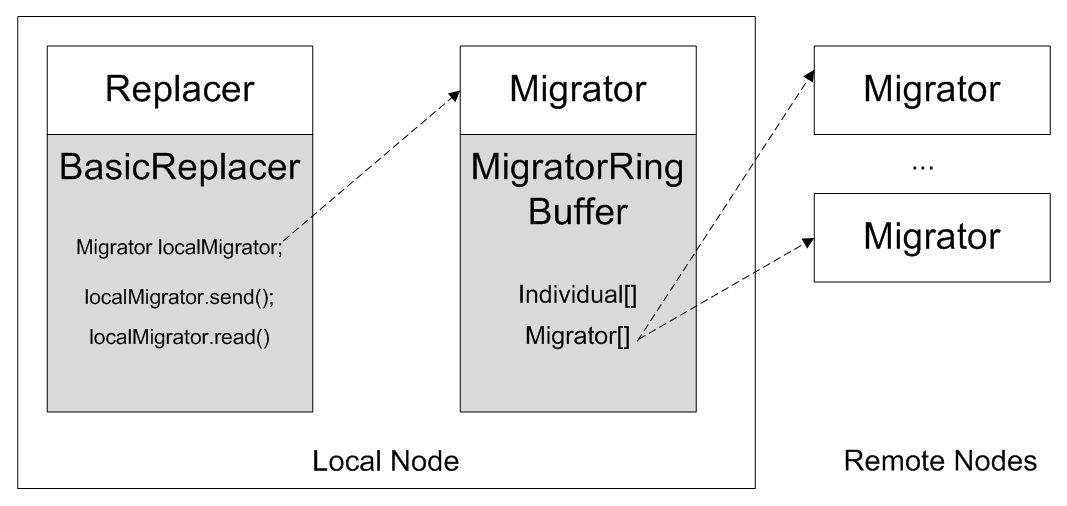
\includegraphics[scale=0.7]{images/migrator.eps}
\end{center} 
\caption{Using the Migrator service to create a distributed island EA with a ring topology (white boxes are service interfaces and grey boxes are implementations).} 
\label{MIGRATOR} 
\end{figure*} 

\section{Conclusions}
\label{sec:conclusions}
This work shows the requirements to create a service oriented evolutionary framework and the technology used to accomplish these requirements. Service Oriented Architecture (SOA) offers independence of language, distribution or even operating systems, allowing the integration of different elements. However, some issues have to be considered in the development: the services are stateless input/output functions, services can appear or disappear in real time and the order of execution could not be fixed. In the Evolutionary Algorithms (EAs) area, services must be developed taking into account these issues, so the abstract design of elements for EAs has been explained. Technological requirements are also solved using an existent service oriented technology: OSGi. The elements to create a service oriented architecture for EAs using this technology have been described, and an example of development has been shown.

As future work a study about scalability using other algorithms (such as GRASP, Scatter Search, Ant Colony Optimization and others) will be performed. In addition, we are going to increase the usage of the OSGi capabilities, like the Event Administration or automatic service management in a deeper way.
Additionally we intend to create a web portal or a Maven\footnote{\url{http://maven.apache.org}} repository to centralize all new implementations of problems and algorithms to let the distribution within the base platform. A study of porting existing software to our framework (especially those works that are written in Java, like DREAM or ECJ) will be performed. Moreover, due to the ease of implementations binding with their interfaces, it is planned to develop the functionality of choosing one implementation or another depending on several parameters or, for example, using Genetic Programming to evolve and hybridize algorithms.

%ACKNOWLEDGMENTS are optional
\section{Acknowledgments}
This work has been supported in part by FPU research grant AP2009-2942 and projects EvOrq (P08-TIC-03903), Project 83 (CANUBE) awarded by the CEI-BioTIC UGR, and TIN2011-28627-C04-02 (ANYSELF).

%
% The following two commands are all you need in the
% initial runs of your .tex file to
% produce the bibliography for the citations in your paper.


%\bibliographystyle{abbrv} CAMBIAR!!!!!!
%\bibliographystyle{plain} %ESTE
%\bibliography{osgi-evosoft}  % sigproc.bib is the name of the Bibliography in this case
\begin{thebibliography}{10}

\bibitem{MALLBA}
E.~Alba, F.~Almeida, M.~Blesa, C.~Cotta, M.~D{\'i}az, I.~Dorta, J.~Gabarr{\'o},
  C.~Le{\'o}n, G.~Luque, J.~Petit, C.~Rodr{\'i}guez, A.~Rojas, and F.~Xhafa.
\newblock Efficient parallel {LAN/WAN} algorithms for optimization. the
  {MALLBA} project.
\newblock {\em Parallel Computing}, 32(5-6):415--440, 2006.

\bibitem{KEEL}
J.~Alcal{\'a}-Fdez, L.~S{\'a}nchez, S.~Garc\'{\i}a, M.~J. del Jes{\'u}s,
  S.~Ventura, J.~M.~Garrell i~Guiu, J.~Otero, C.~Romero, J.~Bacardit, V.~M.
  Rivas, J.~C. Fern{\'a}ndez, and F.~Herrera.
\newblock {KEEL}: a software tool to assess evolutionary algorithms for data
  mining problems.
\newblock {\em Soft Computing}, 13(3):307--318, 2009.

\bibitem{OPENSCIENCEGRID}
M.~Altunay, P.~Avery, K.~Blackburn, B.~Bockelman, M.~Ernst, D.~Fraser,
  R.~Quick, R.~Gardner, S.~Goasguen, T.~Levshina, M.~Livny, J.~McGee, D.~Olson,
  R.~Pordes, M.~Potekhin, A.~Rana, A.~Roy, C.~Sehgal, I.~Sfiligoi,
  F.~Wuerthwein, and {Open Sci Grid Executive Board}.
\newblock {A Science Driven Production Cyberinfrastructure-the Open Science
  Grid}.
\newblock {\em {Journal of GRID Computing}}, {9}({2, Sp. Iss. SI}):{201--218},
  {JUN} {2011}.

\bibitem{DREAM}
M.G. Arenas, Pierre Collet, A.E. Eiben, M\'ark Jelasity, J.~J. Merelo, Ben
  Paechter, Mike Preu\ss, and Marc Schoenauer.
\newblock A framework for distributed evolutionary algorithms.
\newblock In {\em Parallel Problem Solving from Nature, PPSN VII}, pages
  665--675, 2002.

\bibitem{JMETAL}
J.~J. Durillo, A.~J. Nebro, and E.~Alba.
\newblock The jmetal framework for multi-objective optimization: Design and
  architecture.
\newblock In {\em IEEE Congress on Evolutionary Computation}, pages 1--8, 2010.

\bibitem{GENERICITY05}
C.~Gagn{\'e} and M.~Parizeau.
\newblock Genericity in evolutionary computation software tools: Principles and
  case-study.
\newblock {\em International Journal on Artificial Intelligence Tools},
  15(2):173, 2006.

\bibitem{OSGILIATHNICSO}
P.~Garc{\'\i}a-S{\'a}nchez, J.~Gonz{\'a}lez, P.~Castillo, J.~Merelo, A.~Mora,
  J.~Laredo, and M.~Arenas.
\newblock {A Distributed Service Oriented Framework for Metaheuristics Using a
  Public Standard}.
\newblock {\em Nature Inspired Cooperative Strategies for Optimization (NICSO
  2010)}, pages 211--222, 2010.

\bibitem{OSGILIATH}
P.~Garc{\'i}a-S{\'a}nchez, J.~Gonz{\'a}lez, P.A. Castillo, M.G. Arenas, and
  J.J. Merelo-Guerv{\'o}s.
\newblock Service oriented evolutionary algorithms.
\newblock {\em Soft Computing}, pages 1--17, 2013.
\newblock In press.

\bibitem{GATEWAY}
P.~Garc\'{\i}a-S{\'a}nchez, J.~Gonz{\'a}lez, A.~Miguel Mora, and A.~Prieto.
\newblock Deploying intelligent e-health services in a mobile gateway.
\newblock {\em Expert Syst. Appl.}, 40(4):1231--1239, 2013.

\bibitem{EASYLOCAL}
L.D. Gaspero and A.~Schaerf.
\newblock Easylocal++: an object-oriented framework for the flexible desgin of
  local search algorithms and metaheuristics.
\newblock In {\em Proceedings of 4th Metaheuristics International Conference
  (MIC'2001)}, pages 287--292, 2001.

\bibitem{SIGMA}
J.~R. Gonz\'alez, D.~A. Pelta, and A.~D. Masegosa.
\newblock A framework for developing optimization-based decision support
  systems.
\newblock {\em Expert Systems with Applications}, 36(3, Part 1):4581 -- 4588,
  2009.

\bibitem{OSGICHALLENGES}
P.~Kriens.
\newblock Research challenges for {OSGi}.
\newblock 2008.
\newblock Available at:
  \url{http://www.osgi.org/blog/2008/02/research-challenges-for-osgi.html}.

\bibitem{METCO}
C.~Le\'on, G.~Miranda, and C.~Segura.
\newblock Metco: A parallel plugin-based framework for multi-objective
  optimization.
\newblock {\em International Journal on Artificial Intelligence Tools},
  18(4):569--588, 2009.

\bibitem{PARADISEO}
A.~Liefooghe, L.~Jourdan, and E.G. Talbi.
\newblock {A software framework based on a conceptual unified model for
  evolutionary multiobjective optimization: ParadisEO-MOEO}.
\newblock {\em European Journal of Operational Research}, 2010.

\bibitem{ECJ}
S.~Luke et~al.
\newblock {ECJ: A Java-based Evolutionary Computation and Genetic Programming
  Research System}, 2009.
\newblock Available at \url{http://www. cs. umd. edu/projects/plus/ec/ecj}.

\bibitem{PERL}
J.J. Merelo~Guerv\'os, P.~Castillo, and E.~Alba.
\newblock Algorithm::evolutionary, a flexible {P}erl module for evolutionary
  computation.
\newblock {\em Soft Computing - A Fusion of Foundations, Methodologies and
  Applications}, 14:1091--1109, 2010.

\bibitem{GRIDUFO}
A.~Munawar, M.~Wahib, M.~Munetomo, and K.~Akama.
\newblock The design, usage, and performance of gridufo: A grid based unified
  framework for optimization.
\newblock {\em Future Generation Computer Systems}, 26(4):633 -- 644, 2010.

\bibitem{OSGI}
{OSGi Alliance}.
\newblock {OSGi} service platform release 4.2, 2010.
\newblock Available at: \url{http://www.osgi.org/Release4/Download}.

\bibitem{PAPAZOGLOU}
M.~Papazoglou and W.-J. van~den Heuvel.
\newblock Service oriented architectures: approaches, technologies and research
  issues.
\newblock {\em The VLDB Journal}, 16:389--415, 2007.
\newblock 10.1007/s00778-007-0044-3.

\bibitem{petzold2011dynamic}
M.~Petzold, O.~Ullrich, and E.~Speckenmeyer.
\newblock Dynamic distributed simulation of {DEVS} models on the {OSGi} service
  platform.
\newblock {\em Proceedings of ASIM 2011}, 2011.

\bibitem{HEURISTICLAB}
S.~Wagner and M.~Affenzeller.
\newblock {HeuristicLab: A generic and extensible optimization environment}.
\newblock In {Ribeiro, B. and Albrecht, R.F. and Dobnikar, A. and Pearson, D.W.
  and Steele, N.C.}, editor, {\em {Adaptive and Natural Computing Algorithms}},
  {Springer Computer Science}, pages {538--541}, {2005}.
\newblock {7th International Conference on Adaptive and Natural Computing
  Algorithms (ICANNGA), Coimbra, Portugal, MAR 21-23, 2005}.

\bibitem{PLUGINS}
S.~Wagner, S.~Winkler, E.~Pitzer, G.~Kronberger, A.~Beham, R.~Braune, and
  M.~Affenzeller.
\newblock Benefits of plugin-based heuristic optimization software systems.
\newblock In Roberto Moreno~D{\'i}az, Franz Pichler, and Alexis
  Quesada~Arencibia, editors, {\em Computer Aided Systems Theory - EUROCAST
  2007}, volume 4739 of {\em Lecture Notes in Computer Science}, pages
  747--754. Springer Berlin / Heidelberg, 2007.

\bibitem{GALIB}
B.~M. Wall.
\newblock A genetic algorithm for resource-constrained scheduling, {Ph.D}.
  thesis, {MIT}.
\newblock 1996.
\newblock Available at: \url{http://lancet.mit.edu/ga}.

\end{thebibliography}



\end{document}
